\chapter{Gewöhnliche Differentialgleichungen für dynamische Systeme}
\label{\detokenize{ode/ode:gewohnliche-differentialgleichungen-fur-dynamische-systeme}}\label{\detokenize{ode/ode::doc}}
Wir wollen in diesem Kapitel weiterführende Konzepte zum Thema gewöhnlicher Differentialgleichungen einführen. Hierfür wiederholen wir zunächst die wichtigsten Aussagen und Begriffe, die Sie in Kaptiel 7 {[}{]} kengelernt haben.


\section{Einführung in dynamische Systeme}
\label{\detokenize{ode/motivation:einfuhrung-in-dynamische-systeme}}\label{\detokenize{ode/motivation::doc}}

\subsection{Dynamische Systeme}
\label{\detokenize{ode/motivation:dynamische-systeme}}

\subsection{Gewöhnliche Differentialgleichungen}
\label{\detokenize{ode/motivation:gewohnliche-differentialgleichungen}}
Im folgenden bezeichnet \(U\subset\R^n\) stets eine \textbf{offene} Teilmenge des \(\R^n\)
\label{ode/motivation:def:DGL}
\begin{definition}{}{}



Es sei \(I\subset\R^+_0\) eine offenes Intervall und \(F:I\times U\rightarrow\R^n\) eine \textbf{stetige} Funktion, dann nennen wir
\begin{align}\label{equation:ode/motivation:eq:DGL}
\dot{x}(t) = F(t, x(t))\quad\forall t\in I
\end{align}
gewöhnliche Differentialgleichung (DGL) erster Ordnung. Eine Funktion \(\phi\in C^1(I,\R^n)\) heißt \textbf{Lösung} der DGL, falls gilt,
\begin{align*}
\dot{\phi}(t) = F(t, \phi(t))\quad\forall t\in I.
\end{align*}
Die Menge \(G=I\times U\) wird hier auch als \textbf{erweiterter Phasenraum} bezeichnet.
\end{definition}

Speziell in den nächsten Abschnitten behandeln wir DGLs, für welche die Funktion \(F\) nicht von der Zeit abhängt.
\label{ode/motivation:definition-1}
\begin{definition}{}{}



Hängt die Funktion \(F\) in \cref{ode/motivation:def:DGL}  nicht von der Zeit ab, d.h., wir haben \(F:U\rightarrow\R^n\) dann heiß die Gleichung
\begin{align}\label{equation:ode/motivation:eq:DGL}
\dot{x(t)} = F(x(t))\quad\forall t\in I
\end{align}
\textbf{autonome DGL}.
\end{definition}


\subsection{Anfangswertprobleme}
\label{\detokenize{ode/motivation:anfangswertprobleme}}
Üblicherweise betrachtet man nicht nur DGLs sondern sogenannte Anfangswertprobleme. Hierbei wählt man einen ausgezeichneten Zeitpunkt \(t_0\in I\) aus dem Zeitintervall \(I\) an welchem man die Lösung explizit durch einen Anfangswert \(x_0\in U\) vorgibt. Im Setting von \cref{ode/motivation:def:DGL}  heißt
das Gleichungssystem
\begin{align}\label{equation:ode/motivation:eq:AWP}
\dot{x}(t) = F(t, x(t))\quad\forall t\in I
x(t_0) = x_0
\end{align}
\textbf{Anfangswertproblem}. Sofern nicht explizit angegeben werden wir im folgenden annehmen, dass \(t_0=0\) gilt.


\subsection{Existenz und Eindeutigkeit einer Lösung}
\label{\detokenize{ode/motivation:existenz-und-eindeutigkeit-einer-losung}}
Wir wiederholen die wichtigsten Existenzaussagen zu Anfangswertproblem. Die wichtigste Eigenschaften in diesem Kontext ist die Lipschitzstetigkeit der rechten Seite \(F\).
\label{ode/motivation:definition-2}
\begin{definition}{}{}



\(F\)
\end{definition}


\section{Flüsse und Phasenportraits}
\label{\detokenize{ode/fluesse:flusse-und-phasenportraits}}\label{\detokenize{ode/fluesse::doc}}
In diesem Abschnitt führen wir zunächst grundlegende Konzepte ein und betrachten danach geometrische Interpretation von DGLs.

Untenstehend die wichtigsten Schlagwörter:
\begin{itemize}
\item {} 
Fluss \cref{ode/fluesse:def:Fluss} ,

\item {} 
lokaler Fluss \cref{ode/fluesse:def:LokFluss} ,

\item {} 
Fluss einer DGL,
\begin{itemize}
\item {} 
Bahnkurve,

\item {} 
Orbit,

\item {} 
Ruhelage

\end{itemize}

\end{itemize}


\subsection{Flüsse}
\label{\detokenize{ode/fluesse:flusse}}
Wir beginnen zunächst damit ein wichtiges Konzept einzuführen, welches die Beschreibung zeitabhängiger Systeme vereinfacht. Die folgende Definition ist zunächst sehr allgemein gehalten und wird später für unsere Anwendungen auf DGLs konkretisiert.
\label{ode/fluesse:def:Fluss}
\begin{definition}{}{}



Sei \(U\) eine Menge und \(I=\R^+_0\), dann heißt eine Abbildung \(\Phi:I\times U\rightarrow U\) \textbf{Fluss}, falls gilt,
\begin{enumerate}

\item {} 
\(\Phi(0, x) = x\) für alle \(x\in U\),

\item {} 
\(\Phi(t, \Phi(x,s)) = \Phi(s + t, x)\) für alle \(x\in U\) und alle \(s,t\in I\).

\end{enumerate}

Das Tripel \((I, U, \Phi)\) heißt \textbf{dynamisches System}.
\end{definition}
\label{ode/fluesse:remark-1}
\begin{emphBox}{}{}{Remark 1.1 (Notation)}



Anstatt beide Argument in Klammern wie in obiger Definition zu schreiben, benutzt man häufig folgende Darstellung,
\begin{align*}
\Phi_t(x) = \Phi(t, x).
\end{align*}\end{emphBox}

In unserem Fall wollen wir speziell die Lösungen einer autonomen DGL
\begin{align*}
\dot{x} = F(x).
\end{align*}
für \(F\in C^1(U;\R^n)\) als Fluss interpretieren. Hierbei soll das zweite Argument jeweils den Anfangswert
\(x_0\in U\) angeben und \(\Phi(x_0) = \Phi(\cdot, x_0)\) dann eine Lösung der DGL sein, d.h., \(\frac{\d}{\d t} \Phi(x_0) = F(\Phi(x_0))\).

Nach dem Satz von Picard Lindelöf (Kapitel 7, {[}\hyperlink{cite.references:id7}{Ten21}{]}) wissen wir, dass für jeden Anfangswert \(x_0\in U\) ein \(\epsilon(x_0) >0\) existiert, s.d., es eine eindeutige Lösung \(\phi: [-\epsilon(x_0), \epsilon(x_0)]\) gibt. In diesem Fall wählen wir also \(I(x_0)=[-\epsilon(x_0), \epsilon(x_0)]\). Wir können also nicht wie in \cref{ode/fluesse:def:Fluss}  auf ganz \(\R^+_0\) als Zeitintervall arbeiten. Stattdessen können wir nur Tupel der Form \((x_0, t)\) betrachten, wobei \(x_0\in U\) fixiert ist und \(t\) aus \(I(x_0)\) gewählt werden kann, was wir mithilfe des kartesischen Produkts
\begin{align*}
\{x_0\}\times I(x_0)
\end{align*}
dargestellt werden kann. Dies führt uns auf den Begriff des lokalen Flusses.
\label{ode/fluesse:def:LokFluss}
\begin{definition}{}{}



Sei \(U\) eine Menge und die Menge \(G\subset \R^+_0\times U\) sei gegeben als
\begin{align*}
G = \bigcup_{x\in U} \{x\}\times I(x),
\end{align*}
wobei \(0\in I(x)\subset \R^+_0\) für jedes \(x\in U\).

Dann heißt eine Abbildung \(\Phi: G\rightarrow U\) \textbf{lokaler Fluss}, falls
\begin{enumerate}

\item {} 
\(\Phi(0,x) = x\) für alle \(x\in U\),

\item {} 
\(\Phi(t, \Phi(s, x)) = \Phi(s+t, x)\) für alle \(x\in U\) und alle \(s,t\) s.d. \(s, s+t\in I(x)\) und \(t\in I(\Phi(x,s))\).

\end{enumerate}
\end{definition}

Im nächsten Lemma wollen wir nun sehen, dass die Lösung einer DGL tatsächlich als lokaler Fluss interpretiert werden kann.
\label{ode/fluesse:lemma-3}
\begin{lemma}{}{}



Sei \(U\subset\R^n\), \(F:U \rightarrow \R^n\) lokal Lipschitz stetig, dann existieren Intervalle \(I(x_0)\), sodass es für
\begin{align*}
G = \bigcup_{x_0\in U} I(x_0)\times\{x_0\},
\end{align*}
eine Funktion \(\Phi:G\rightarrow \R^n\) gibt, mit folgenden Eigenschaften
\begin{enumerate}

\item {} 
\(\frac{\d}{\d t} \Phi(t, x_0) = F(\Phi(t, x_0))\) für alle \((t,x_0)\in G\),

\item {} 
\(\Phi\) ist ein lokaler Fluss auf \(G\).

\end{enumerate}
\end{lemma}
\label{ode/fluesse:remark-4}
\begin{emphBox}{}{}{Remark 1.2}



Die Abbildung \(\Phi\) bezeichnet man hier auch als\textbf{Fluss einer DGL}.
\end{emphBox}

\begin{proof}
 Nach dem Satz von Picard Lindelöf existiert für jedes \(x_0\in U\) ein \(\epsilon(x_0)>0\) s.d., die Lösung der DGL
auf \([-\epsilon(x_0),\epsilon(x_0)]\) mit AW \(x_0\) existiert. Daher können wir
\begin{align*}
G = \bigcup_{x_0\in U} [-\epsilon(x_0),\epsilon(x_0)] \times\{x_0\}
\end{align*}
wählen und \(\Phi\) so definieren, dass
\begin{align*}
\frac{\d}{\d t} \Phi(t, x_0) &= F(\Phi(t, x_0))\\
\Phi(0, x_0) &= x_0
\end{align*}
für alle \((t, x_0)\in G\). Damit haben wir 1. und die erste Flusseigenschaft gezeigt. Die zweite Flusseigenschaften ist eine direkte Folgerung aus der Eindeutigkeit der Lösung der DGL. Wir führen den Beweis trotzdem explizit aus. Es sei \(x_0\in U, s\in [-\epsilon(x_0), \epsilon(x_0)]\) und weiterhin \(t\), s.d., \(s+t \in [-\epsilon(x_0), \epsilon(x_0)]\) und \(t\in [-\epsilon(\Phi(s,x_0)), \epsilon(\Phi(s,x_0))]\).
Per Definition löst die Funktion
\begin{align*}
\phi_1(\tau) := \Phi(s + \tau, x_0)
\end{align*}
sowie auch die Funktion
\begin{align*}
\phi_2(\tau) := \Phi(\tau, \Phi(s,x_0))
\end{align*}
die DGL auf dem Intervall \([t, \epsilon(x_0)]\). Weiterhin wissen wir, dass
\begin{align*}
\phi_1(0) = \Phi(s, x_0) = \Phi(0, \Phi(s, x_0)) = \phi_2(0),
\end{align*}
somit stimmen also beide Funktionen an einem Punkt überein und sind somit schon auf dem gesamten Intervall \([t, \epsilon(x_0)]\) gleich, was
eine Folgerung aus dem Eindeutigkeitssatz ({[}\hyperlink{cite.references:id7}{Ten21}{]}, Kapitel 7) ist. Wir haben also
\begin{align*}
\Phi(s + \tau, x_0) = \phi_1(\tau) = \phi_2(\tau) = \Phi(\tau, \Phi(s,x_0))
\end{align*}
für jedes \(\tau\in [t, \epsilon(x_0)]\).
\end{proof}


\subsection{Phasenportraits}
\label{\detokenize{ode/fluesse:phasenportraits}}
Die teilweise abstrakten Begriffe zu Flüssen werden nun mit einfachen geometrische Anschauung unterlegen. Dafür benötigen wir zunächst die folgenden Definitionen.
\label{ode/fluesse:definition-5}
\begin{definition}{}{}



Es sei \(\Phi:G\rightarrow U\) ein Fluss einer DGL, mit \(G\subset \R^+_0\times U\).
\begin{itemize}
\item {} 
Für jedes \(x_0\in U\) heißt die Funktion \(t\mapsto \Phi(t, x_0)\) \textbf{Bahnkurve} durch \(x_0\).

\item {} 
Die Menge \(\mathcal{O}(x_0) := \{\Phi(t, x_0): (t, x_0)\in G\}\) heißt \textbf{Orbit} oder \textbf{Trajektorie} durch \(x_0\).

\item {} 
Ein Orbit heißt \textbf{Ruhelage}, falls \(\mathcal{O}(x_0) = \{x_0\}\).

\item {} 
Ein Anfangswert \(x_0\in U\) heißt \textbf{periodisch} mit Periode \(T>0\), falls \(\Phi(T, x_0) = x_0\).

\end{itemize}
\end{definition}
\label{ode/fluesse:example-6}
\begin{example}{}{}



Die Bewgeungsgeleichung für den harmonischen Oszillator is gegeben durch
\begin{align*}
r~\ddot{x}(t) + m~\dot{x}(t) + k~x(t)=0
\end{align*}
hierbei ist
\begin{itemize}
\item {} 
\(x(t)\) die horizontale Auslenkung zum Zeitpunkt \(t\),

\item {} 
\(m\) die Masse des Objekts,

\item {} 
\(r\) die Dämpfungskonstante,

\item {} 
\(k\) die Federkonstante.

\end{itemize}

Durch einführung der Variable \(p(t):= m~\dot{x}(t)\) als Impuls erhalten wir das System von DGLs
\begin{align*}
\dot{x}(t) &= \frac{1}{m}~p(t) \\
\dot{p}(t) &= -k~x(t) - \frac{r}{m}~p(t).
\end{align*}
Betrachten wir speziell den ungedämpften Fall, \(r=0\), erhalten wir zum Anfangswert \((x,p)\) die Lösung
\begin{align*}
\Phi(t, (x,p)) = 
\begin{pmatrix}
\frac{p}{\omega m}\sin(\omega t) + x~\cos(\omega t)\\
p \cos(\omega t) - m x \sin(\omega t)
\end{pmatrix}
\end{align*}
wobei \(\omega=\sqrt{\frac{k}{m}}\) die Eigenfrequenz des Systems ist.
\end{example}


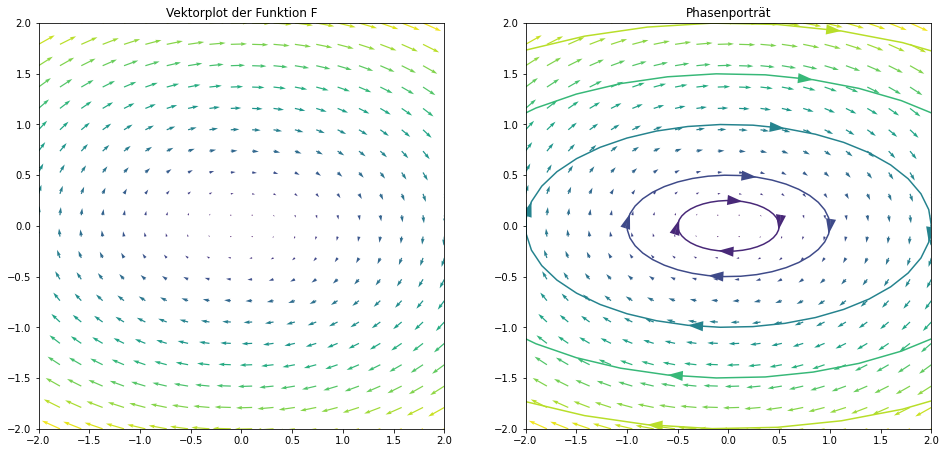
\includegraphics{{C:/Tim/Uni/Lectures/MathePhysikerC/_build/jupyter_execute/fluesse_1_0}.png}


\section{Hamiltonsche Differentialgkeichungen und Phasenportraits}
\label{\detokenize{ode/hamilton:hamiltonsche-differentialgkeichungen-und-phasenportraits}}\label{\detokenize{ode/hamilton::doc}}
Ein wichtiges Prinzip für viele physikalischen Anwendungen sind Erhaltungssätze und die dazugehörigen Erhaltungsgrößen. Aus der klassichen Mechanik kennen wir z.B.
\begin{itemize}
\item {} 
Energieerhaltung,

\item {} 
Impulserhaltung.

\end{itemize}

In ?? haben wir Bewegungslgleichungen als System von DGLs hergeleitet und gelöst, deshalb wollen wir nun die nötige Theorie entwickeln, die es uns erlaubt Erhaltungsgrößen direkt aus der DGL Formulierung zu erhalten.
\label{ode/hamilton:example-0}
\begin{example}{}{}


\end{example}


